\documentclass[aspectratio=169,19pt,english]{beamer}

% =========================================================
\usetheme{Berkeley}
\usecolortheme{default}

\definecolor{PythonBlue}{HTML}{306998}
\definecolor{PythonYellow}{HTML}{FFD43B}
\definecolor{DeepNavy}{HTML}{14213D}
\definecolor{SoftWhite}{HTML}{F7F9FC}
\definecolor{CodeGreen}{HTML}{2A9D8F}

\setbeamercolor{structure}{fg=PythonBlue}
\setbeamercolor{palette primary}{bg=DeepNavy,fg=white}
\setbeamercolor{palette secondary}{bg=PythonBlue,fg=white}
\setbeamercolor{palette tertiary}{bg=DeepNavy,fg=white}
\setbeamercolor{palette quaternary}{bg=PythonBlue,fg=white}
\setbeamercolor{title}{fg=white,bg=DeepNavy}
\setbeamercolor{frametitle}{fg=white,bg=DeepNavy}
\setbeamercolor{block title}{fg=white,bg=PythonBlue}
\setbeamercolor{block body}{fg=DeepNavy,bg=SoftWhite}
\setbeamercolor{alerted text}{fg=PythonBlue}
\setbeamercolor{normal text}{fg=DeepNavy,bg=white}
\setbeamercolor{item}{fg=PythonBlue}
\setbeamercolor{section in toc}{fg=PythonBlue}
\setbeamercolor{bloqueder}{bg=red!20, fg=black}
\setbeamercolor{bloquetitder}{bg=red, fg=white}

\setbeamercolor{bloqueizq}{bg=blue!20, fg=black}
\setbeamercolor{bloquetitizq}{bg=blue, fg=white}
\setbeamertemplate{navigation symbols}{}
\setbeamertemplate{items}[triangle]
\setbeamertemplate{blocks}[rounded][shadow=false]


\setbeamercovered{invisible}

% =========================================================
% PACKAGES
% =========================================================
\usepackage[T1]{fontenc}
\usepackage[utf8]{inputenc}
\usepackage{babel}
\usepackage{lmodern}
\usepackage{microtype}
\usepackage{enumitem}
\usepackage{graphicx}
\usepackage{booktabs}
\usepackage{mathtools}
\usepackage{amssymb}
\usepackage{xcolor}
\usepackage{listings}
\usepackage{tikz}
\usepackage{hyperref}
\usepackage{listings}
% =========================================================
% PYTHON CODE STYLE
% =========================================================
\lstdefinestyle{pythonstyle}{
	language=Python,
	basicstyle=\ttfamily\small,
	keywordstyle=\color{PythonBlue}\bfseries,
	stringstyle=\color{CodeGreen},
	commentstyle=\color{gray}\itshape,
	numbers=left,
	numberstyle=\tiny\color{gray},
	numbersep=8pt,
	showstringspaces=false,
	breaklines=true,
	frame=single,
	rulecolor=\color{PythonBlue!25},
	backgroundcolor=\color{SoftWhite},
	tabsize=4,
	keepspaces=true,
	columns=fullflexible
}
\lstset{style=pythonstyle}

% =========================================================
% metadata
% =========================================================
\title[CLASS 2.]{Introduction to Programming}
\subtitle{Python Fundamentals}
\author[ ]{Luis Ángel Bustos Ochoa}
\institute{Applied Physics}
\date{\today}

% =========================================================
% DOCUMENT
% =========================================================
\begin{document}
	
	% ---------------------------------------------------------
	% FRAME 1 — TITLE PAGE  ---------------------------------------------------------
	{
		\setbeamercolor{background canvas}{bg=DeepNavy}
		\begin{frame}[plain]
			\centering
			\vspace{0.7cm}
			
			{\color{PythonYellow}\rule{0.22\textwidth}{2pt}}
			
			\vspace{0.65cm}
			
			{\color{white}\Huge\bfseries Introduction To Programming\par}
			
			\vspace{0.35cm}
			
			{\color{PythonYellow}\Large Python fundamentals\par}
			
			\vspace{0.8cm}
			
			\begin{tikzpicture}
				\node[
				rounded corners=8pt,
				fill=white,
				text=PythonBlue,
				inner sep=14pt
				] {
					\begin{minipage}{0.58\textwidth}
						\centering
						\ttfamily\Large
						Universidad...
					\end{minipage}
				};
			\end{tikzpicture}
			
			\vfill
			
			{\color{white}\large Luis Ángel Bustos Ochoa\par}
			\vspace{0.15cm}
			{\color{white!75}\normalsize Class 2 \textbar{} Course: \par}
			
			\vspace{0.55cm}
			{\color{PythonYellow}\rule{0.22\textwidth}{2pt}}
			
			\vspace{0.35cm}
			{\color{white!70}\small\insertdate\par}
		\end{frame}
	}	
	%
	\section{Fundamentals}
{\Large
	\begin{frame}{Today's Goals}

		\begin{itemize}
			\item[--] Fundamentals 
			%\item Algorithms 
			\item[--] Type of Variables 
			\item[--] Some Exercises 
			
		\end{itemize}
	\end{frame}

\begin{frame}{Fundamentals}
  \textbf{Computers are obedient, not smart}. They do exactly what you tell them to do, word for word, step by step—even if your instructions lead to a error.\\
  An \textbf{algorithm} is a precise, step-by-step set of instructions designed to solve a specific problem or complete a task. 
\end{frame}

\begin{frame}{Fundamentals}
	\framesubtitle{Computers Do What You Tell Them.}
	Think a computer of a kitchen assistant.If you tell it to "cook a complex dish". It will freeze because it doesn't know what that means. But if you give it a step-by-step recipe like: "chop 5 tomatoes, blend for 10 seconds, add 2 grams of salt", it will do it very quickly; because it moves at millions of operations per second.
	
	
\end{frame}
\begin{frame}{You Should Be Familiar With...}
	\framesubtitle{The Concept Of: }
	\begin{itemize}[label=$\diamond$]
		\item Variable 
		\item True/false statements
		\item Connecting statements (or,and, not)
		\item Making decisions (if ... then)
		\item Following flowcharts 
	\end{itemize}
	
\end{frame}
\begin{frame}{If you shouldn't be familiar with the Flowcharts}
	\framesubtitle{You should be familiar with following a set of instructions and making branching desicions.}
	\begin{figure}
		\centering
		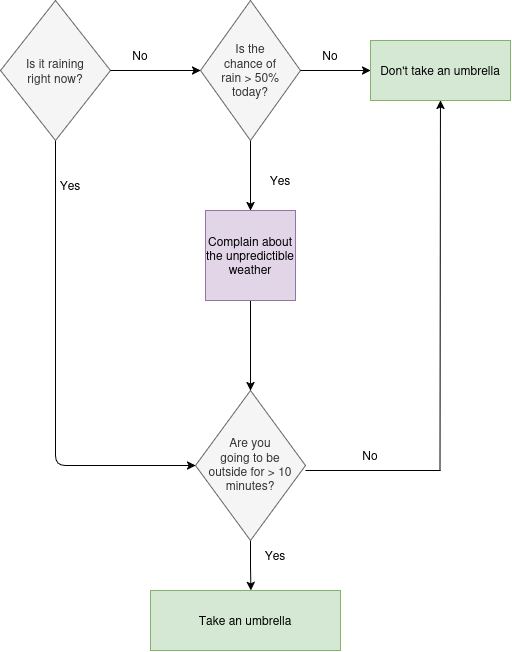
\includegraphics[width=6.9cm, height=6.55cm]{diagram.png}
	
	\end{figure}
	
\end{frame}
\begin{frame}{The structured program theorem}
	\framesubtitle{States that any computable algorithm can be expressed only with three logic control structures.}
\begin{itemize}[label=$\circ$]
	\item Sequence or simple action: Executing one instruction after another in a specific, linear order.
	\item Conditional: valuating a boolean condition to "choose the correct path".
	\item Loop or iteration: Repeating a block of instructions as long as a certain condition remains true.
\end{itemize}
\end{frame}
\section{Variables}
\begin{frame}{Variables}
	The \texttt{=} operator executes a \textbf{right-to-left assignment} (evaluating the right side first, then binding to the left name), not an algebraic equivalence.
	\vspace{0.1cm}
	
	\begin{columns}[t]
		% LEFT COLUMN (RED - MISTAKES & INVALID PATTERNS)
		\begin{column}{0.48\textwidth}
			\setbeamercolor{block title}{use=bloquetitder, bg=bloquetitder.bg, fg=bloquetitder.fg}
			\setbeamercolor{block body}{use=bloqueder, bg=bloqueder.bg, fg=bloqueder.fg}
			\begin{block}{❌ Pitfalls \& Invalid Code}
				\begin{itemize}
					\small{
					\item \textbf{Math equivalence}: Treating \texttt{=} as static math logic (\texttt{a + x = b} throws \texttt{SyntaxError}).
					
					\item \textbf{Syntax violations}: Starting with numbers (\texttt{1st = 5}), spaces, or overriding keywords (\texttt{print = 10}).
					\item \textbf{Single-letter cryptics}: Using \texttt{x}, \texttt{t}, \texttt{p} without domain context.}
				\end{itemize}
			\end{block}
		\end{column}
		
		% RIGHT COLUMN (BLUE - MECHANISMS & CLEAN CODE)
		\begin{column}{0.48\textwidth}
			\setbeamercolor{block title}{use=bloquetitizq, bg=bloquetitizq.bg, fg=bloquetitizq.fg}
			\setbeamercolor{block body}{use=bloqueizq, bg=bloqueizq.bg, fg=bloqueizq.fg}
			\begin{block}{✔ Correct Model \& Standards}
				
				\begin{itemize}
					\small{
					\item \textbf{Right-to-left binding}: \texttt{x = x + 1} evaluates the new value first, then moves the name tag.
					\item \textbf{Valid naming}: Letters or underscores (\texttt{\_}), case-sensitive (\texttt{age} $\neq$ \texttt{Age}).
					\item \textbf{Style}: Descriptive \texttt{snake\_case} names (\texttt{circle\_area}), $<80$ chars/line.}
				\end{itemize}
			\end{block}
		\end{column}
	\end{columns}
\end{frame}

\begin{frame}{Exercise}
	\framesubtitle{"Allowed, Incorrect, Good Variables Names"}
	\begin{enumerate}[label=\arabic*.-]
	\item customer\_list 
	\item print (where this word is a color other than black in Spyder) 
	\item list\_of\_things\_I\_need\_to\_pick\_up\_from\_the\_store 
	\item \%score 
	\item 1 
	\item A
\end{enumerate}
	
\end{frame}
 \section{Primatives}
\begin{frame}
	You'll be able to:
	\begin{itemize}
		\item[*] Write code that creates various types of objects
		\item[*] Write simple lines of codes to manipulate Python variables
	\end{itemize}
\end{frame}
\begin{frame}{Imagine...}
	\framesubtitle{A family made up of:}
\begin{itemize}
	\item[+] 4 people
	\item[+] 3 dogs
	\item[+] 2 cats 
\end{itemize}
Every Person, cat, dog is a separate object (variable)\\
Characteristics are called data \textit{attributes} or \textit{values} for every type
	
\end{frame}
\begin{frame}{Types}
	In the most programming languages few types of objects are basic building blocks for each language. These types are the 'primitives'.
    Python has five basic types (primatives) of objects: 
    \begin{enumerate}[label=\roman*.]
    	\item Integers.
    	\item Floats. 
    	\item Booleans.
    	\item Strings. 
    	\item A special type that represents the absence of a value .
    \end{enumerate}
\end{frame}


\begin{frame}{Integers}
	Objects whose values are real whole numbers (1,0,3,5,-4,-100000).\vspace{0.1cm}
   \fbox{	You do on numbers what you do in math class.}
\end{frame}
\begin{frame}{Floats}
	An object of type floating point (float type) object whose values are decimal numbers. Example: 
	\begin{enumerate}[label=\roman*.]
		\item 0.0
		\item 2.3
		\item -22.8
	\end{enumerate}
\end{frame}
\begin{frame}{Boolean}
	You need to work with more than just numbers. 
	A boolean is a type that only has two possibles vales, \textit{true} or \textit{false}
\end{frame}
\begin{frame}{Strings}
	A string is a sequence of characters surrounded by quotation marks. For example: 'hello', "We're #1!", 'Hi!'
\end{frame}
\begin{frame}{Absence of a value}
	The value is None. Because in python everything is an object, this None also has a type, NoneType. It appear when in a list of variables the value is null.  
\end{frame}
\begin{frame}{converting between different types}
When you are writing a program, each line of code is called a statement. if you want to know what kind of data type is an object, you should use \textit{\textbf{type()}}.\\
And if you want to change the type to another kind of data, use: int(), float(), str().
\end{frame}
\section{exercise}
\begin{frame}{Exercise}
	\begin{alertblock}{Homework}
		write 2 programs in python. Start with a variable that contains the number of minutes (121,361). 
		Your Program should show the results in the following ways:\\
		the first program (121 minutes): \\
		Hours \\
		(number of hours)\\
		Minutes\\
		(number of minutes)
		\\
		The second program (361 minutes):
		361 minutes its equal to (hours) and (minutes) in one line.
	\end{alertblock}
\end{frame}
}
\end{document}